% --------------------------------------------------------------
%                       Initialize
% --------------------------------------------------------------

\documentclass{beamer}


\usepackage{mathHW}
% contains special macros for math environment:
%     unit, p, set, abs, floor, ceil, vec, norm, inner, kernel
% contains special environments for homework:
%     hwproblem, hwsolution
% contains special macros for homework:
%     hwprob, hwanswer, hwplaceholder
% contains useful all-purpose macros:
%     n, lessSeparation, append

\usepackage{multicol}

\usepackage[linesnumbered,ruled,vlined]{algorithm2e}

\usepackage{biblatex}
\bibliography{references}


\newcommand{\dfn}[1]{\alert{\textit{#1}}} % definition of a word
\newcommand{\drp}[1]{\text{DRP}(#1)}
\newcommand{\comdrp}[1]{\text{ComDRP}(#1)}
\newcommand{\optdrp}[1]{\text{OptDRP}(#1)}
\newcommand{\candrp}[1]{\text{CanDRP}(#1)}

\newcommand{\closure}[1]{\left<#1\right>}

\def\matroid{\mathcal{M}}
\def\RR{\mathbb{R}}


\newtheorem{openproblem}{\sffamily Open Problem}
\newtheorem{conjecture}{\sffamily Conjecture}


% --------------------------------------------------------------
%                        Beamer Setup
% --------------------------------------------------------------


% \usetheme{CambridgeUS}

\usetheme{Berkeley}
\usecolortheme{dolphin}

% \definecolor{myorange}{RGB}{255,193,150}
% \definecolor{myorange}{RGB}{231,165,85}
% \mode<presentation>
%  {
%  \usetheme{Berkeley}
%  \usecolortheme{dolphin}
%  \setbeamercolor*{palette secondary}{use=structure,fg=white,bg=myorange}
%  % \setbeamercolor*{palette tertiary}{use=structure,fg=white,bg=green}
%  }


\setbeamerfont{footnote}{size=\tiny}

\beamertemplatenavigationsymbolsempty

\setbeamertemplate{itemize items}[circle]
\setbeamertemplate{enumerate items}[circle]

\setbeamertemplate{section in toc}[circle]
% \setbeamertemplate{subsection in toc}[circle]
% \AtBeginSubsection[]
% {
%   \begin{frame}<beamer>
%     \frametitle{Outline}
%     \tableofcontents[currentsection,currentsubsection]
%   \end{frame}
% }
\AtBeginSection[]
{
  % \begin{frame}<beamer>
  %   \frametitle{Outline}
  %   \tableofcontents[
  %       sectionstyle=show/shaded,
  %       subsectionstyle=show/show/shaded
  %   ]
  % \end{frame}
}


% --------------------------------------------------------------
%                           Title
% --------------------------------------------------------------

\title[Canonical\\Decomposition]{Canonical decomposition of independent graphs with application to materials modeling}

\author[Troy Baker]{Troy Baker\\
PhD Student, Computer Science\\
\n
\footnotesize Joint work\footfullcite{baker2015arxiv} with: Meera Sitharam, Menghan Wang, Joel Willoughby}

\institute{University of Florida}

\date{July 12, 2015}



% --------------------------------------------------------------
%                    Beginning of Document
% --------------------------------------------------------------

\begin{document}


% --------------------------------------------------------------
%                           Body
% --------------------------------------------------------------


\begin{frame}
    \titlepage
\end{frame}


\begin{frame}{Motivation}
    % Motivating problem: Given a geometric constraint system, find a realization of every maximal rigid component in $\RR^d$ satisfying the constraints.
    %
    % Deceptively simple
    Motivating problem: Given a linkage, find a realization in $\RR^2$ satisfying the bar-lengths (for every maximal rigid component).
\n
    Directly solving the quadratic system of bar-length equations takes \alert{double exponential time}.
    % Try k_33 on maple, it won't return a solution any time soon.
\n
    Informally, an \alert{optimal decomposition-recombination (DR-) plan} is a \alert{recursive} decomposition of the graph
    % of the linkage
    into the smallest number of rigid subgraphs.
\n
    This is a \alert{purely combinatorial problem}, that generalizes to any abstract rigidity matroid (and other rigidity-related matroids\footfullcite{Haller2012385}).
\end{frame}

\begin{frame}{DR-Plan}
    \begin{definition}
        A \dfn{decomposition-recombination \mbox{(DR-)} plan} \footfullcite{hoffman2001decompositionI} of graph $G$ is defined as a forest that has the following properties:
        \begin{enumerate}
            \item Each node represents a rigid subgraph of $G$.
            \item A root node is a vertex-maximal rigid subgraph of $G$.
            \item A node is the subgraph of $G$ induced by the union of its children.
            \item A leaf node is a single edge.
        \end{enumerate}
    \end{definition}
\end{frame}


% \begin{frame}{DR-Plan}
%     \begin{definition}
%     % [\dfn{Decomposition-recombination \mbox{(DR-)} plan}]
%         The \dfn{decomposition-recombination \mbox{(DR-)} plan} of a graph $G = (V, E)$ with abstract rigidity matroid $\matroid = (K(V), \closure{\cdot})$ is defined as a forest that has the following properties:
%         \begin{enumerate}
%             % \item Each node, $F$, represents a subset of $E$ such that the subgraph $(V(F), F)$ is rigid (i.e.\ $F\subseteq E$ and $\closure{F} = K(V(F))$.)
%             \item Each node, $F$, represents a rigid subset of $E$ (i.e.\ $F\subseteq E$ and $\closure{F} = K(V(F))$.)
%             % \item A root node induces a vertex-maximal rigid subgraph of $G$.
%             \item A root node induces a maximal subset of $V$.
%             \item The union of the children of $F$ induces  exactly the set $V(F)$.
%             \item A leaf node is a single edge.
%             % (i.e.\ $|F|=1$.)
%         \end{enumerate}
%     \end{definition}
% \end{frame}

\begin{frame}{Optimal DR-Plan}
    \begin{definition}
        A DR-plan is \dfn{optimal} if it minimizes the maximum fan-in over all nodes in the forest.
    \end{definition}

    \begin{figure}\centering
        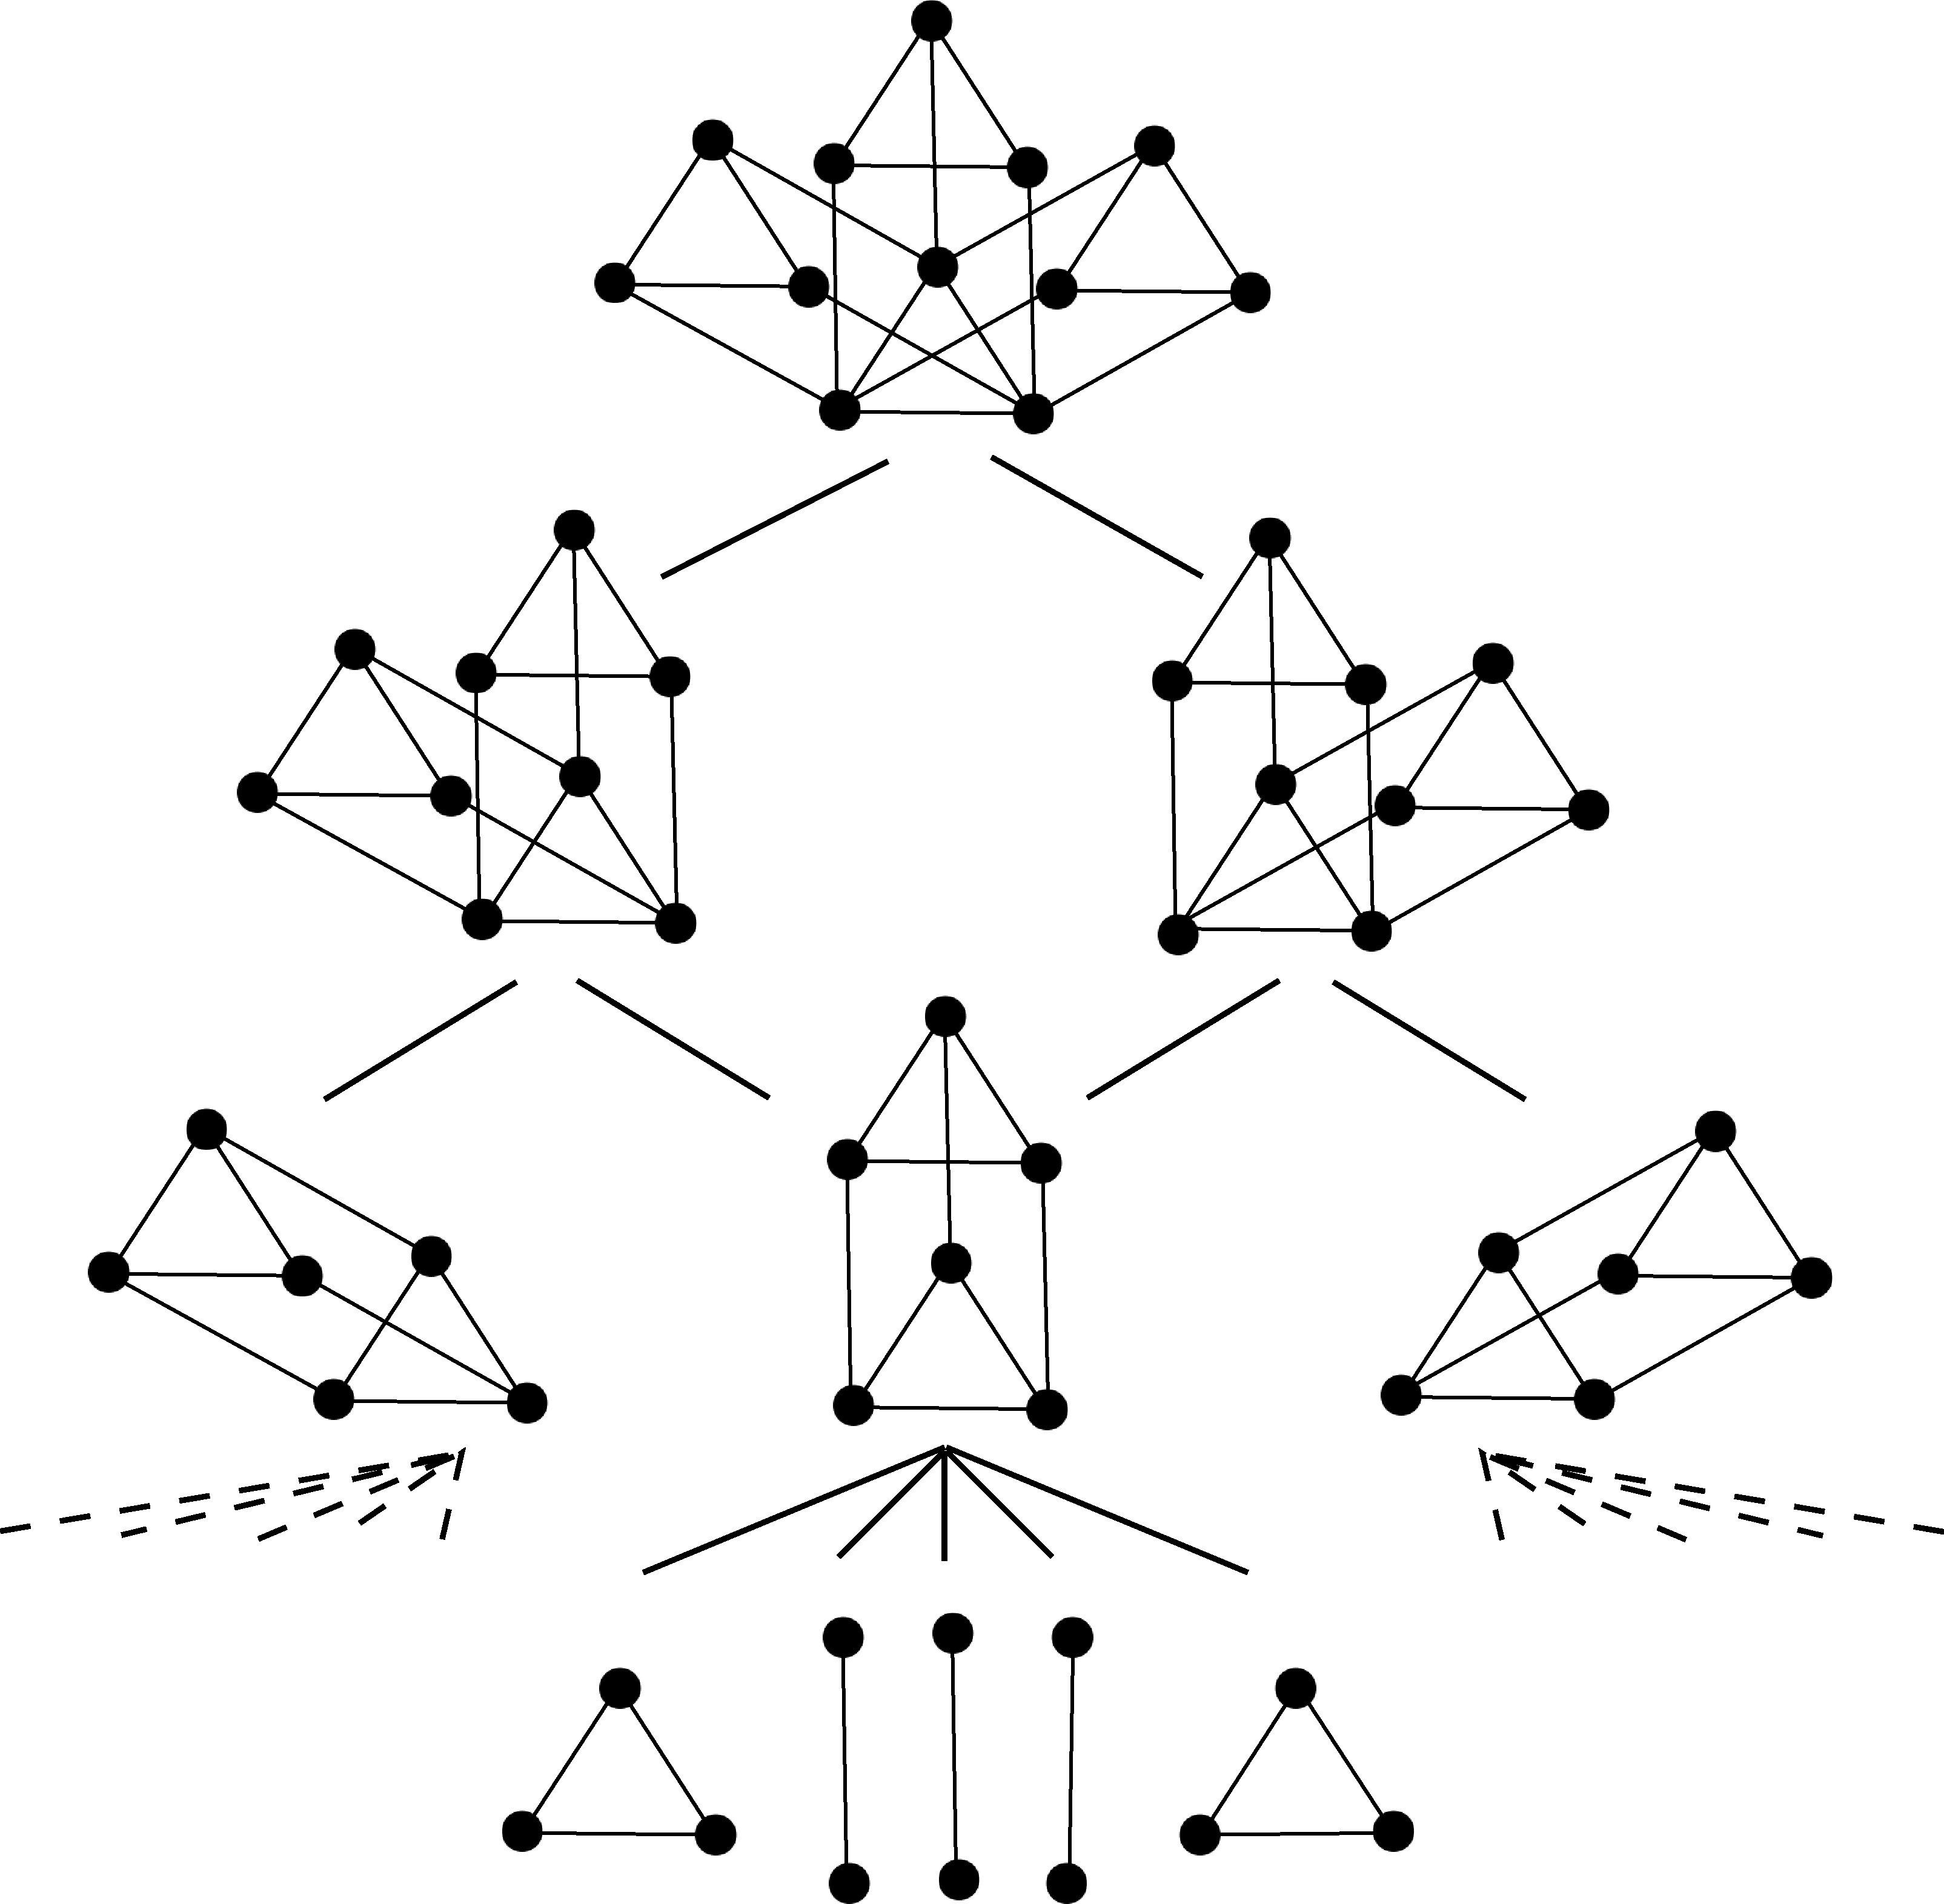
\includegraphics[width=.5\linewidth]{../../img/svg/3xc2c3_candrp_full}
    \end{figure}
\end{frame}

\begin{frame}{Optimal DR-Plan}
    \small
    % Finding an optimal DR-plan is NP-hard in general (even for the usual bar-joint 2D rigidity matroid.)\footfullcite{lomonosov2004graph}

    If the graph is not independent, finding an optimal DR-plan is NP-hard in most cases, \emph{even} if rigidity is captured by an underlying sparsity condition
    % permitting the use of pebble games
    (as in 2D bar-joint.)\footfullcite{lomonosov2004graph}

    \begin{figure}\centering
        \begin{subfigure}{.35\linewidth}\centering
            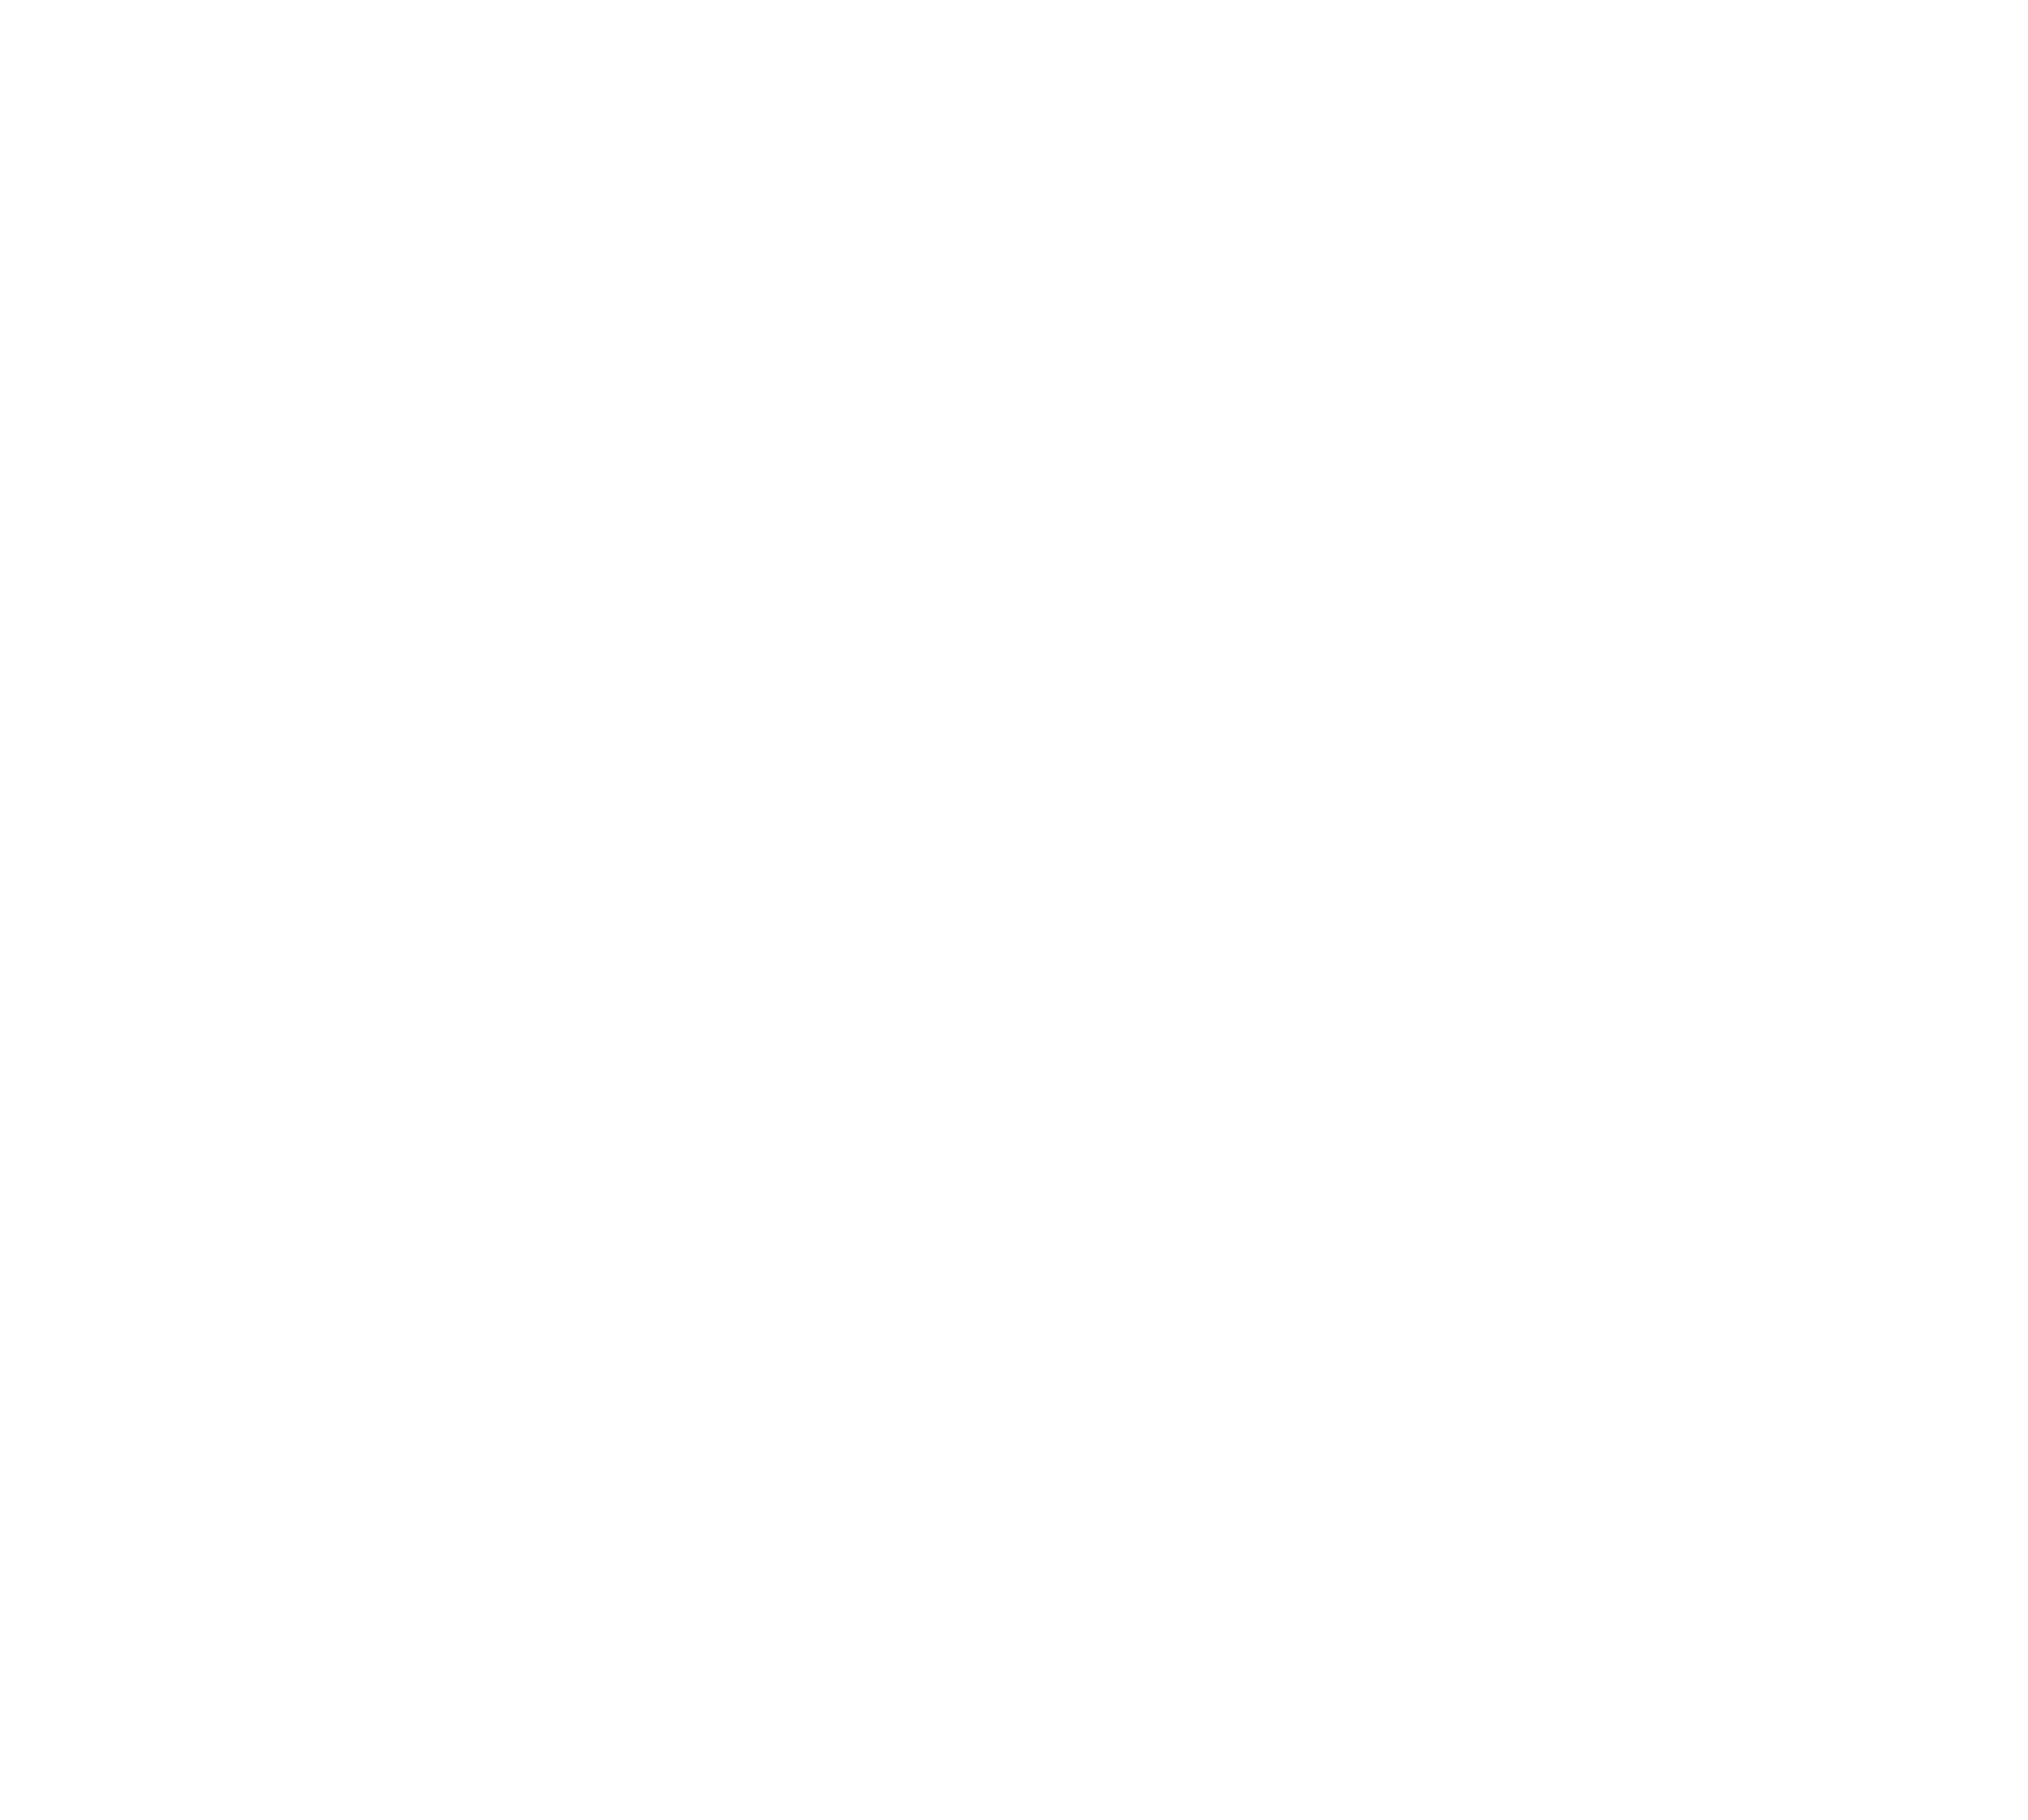
\includegraphics[width=\linewidth]{../../img/svg/new_overconstrained_optimal}
        \end{subfigure}
        %
        \hspace{.1\linewidth}
        \begin{subfigure}{.35\linewidth}\centering
            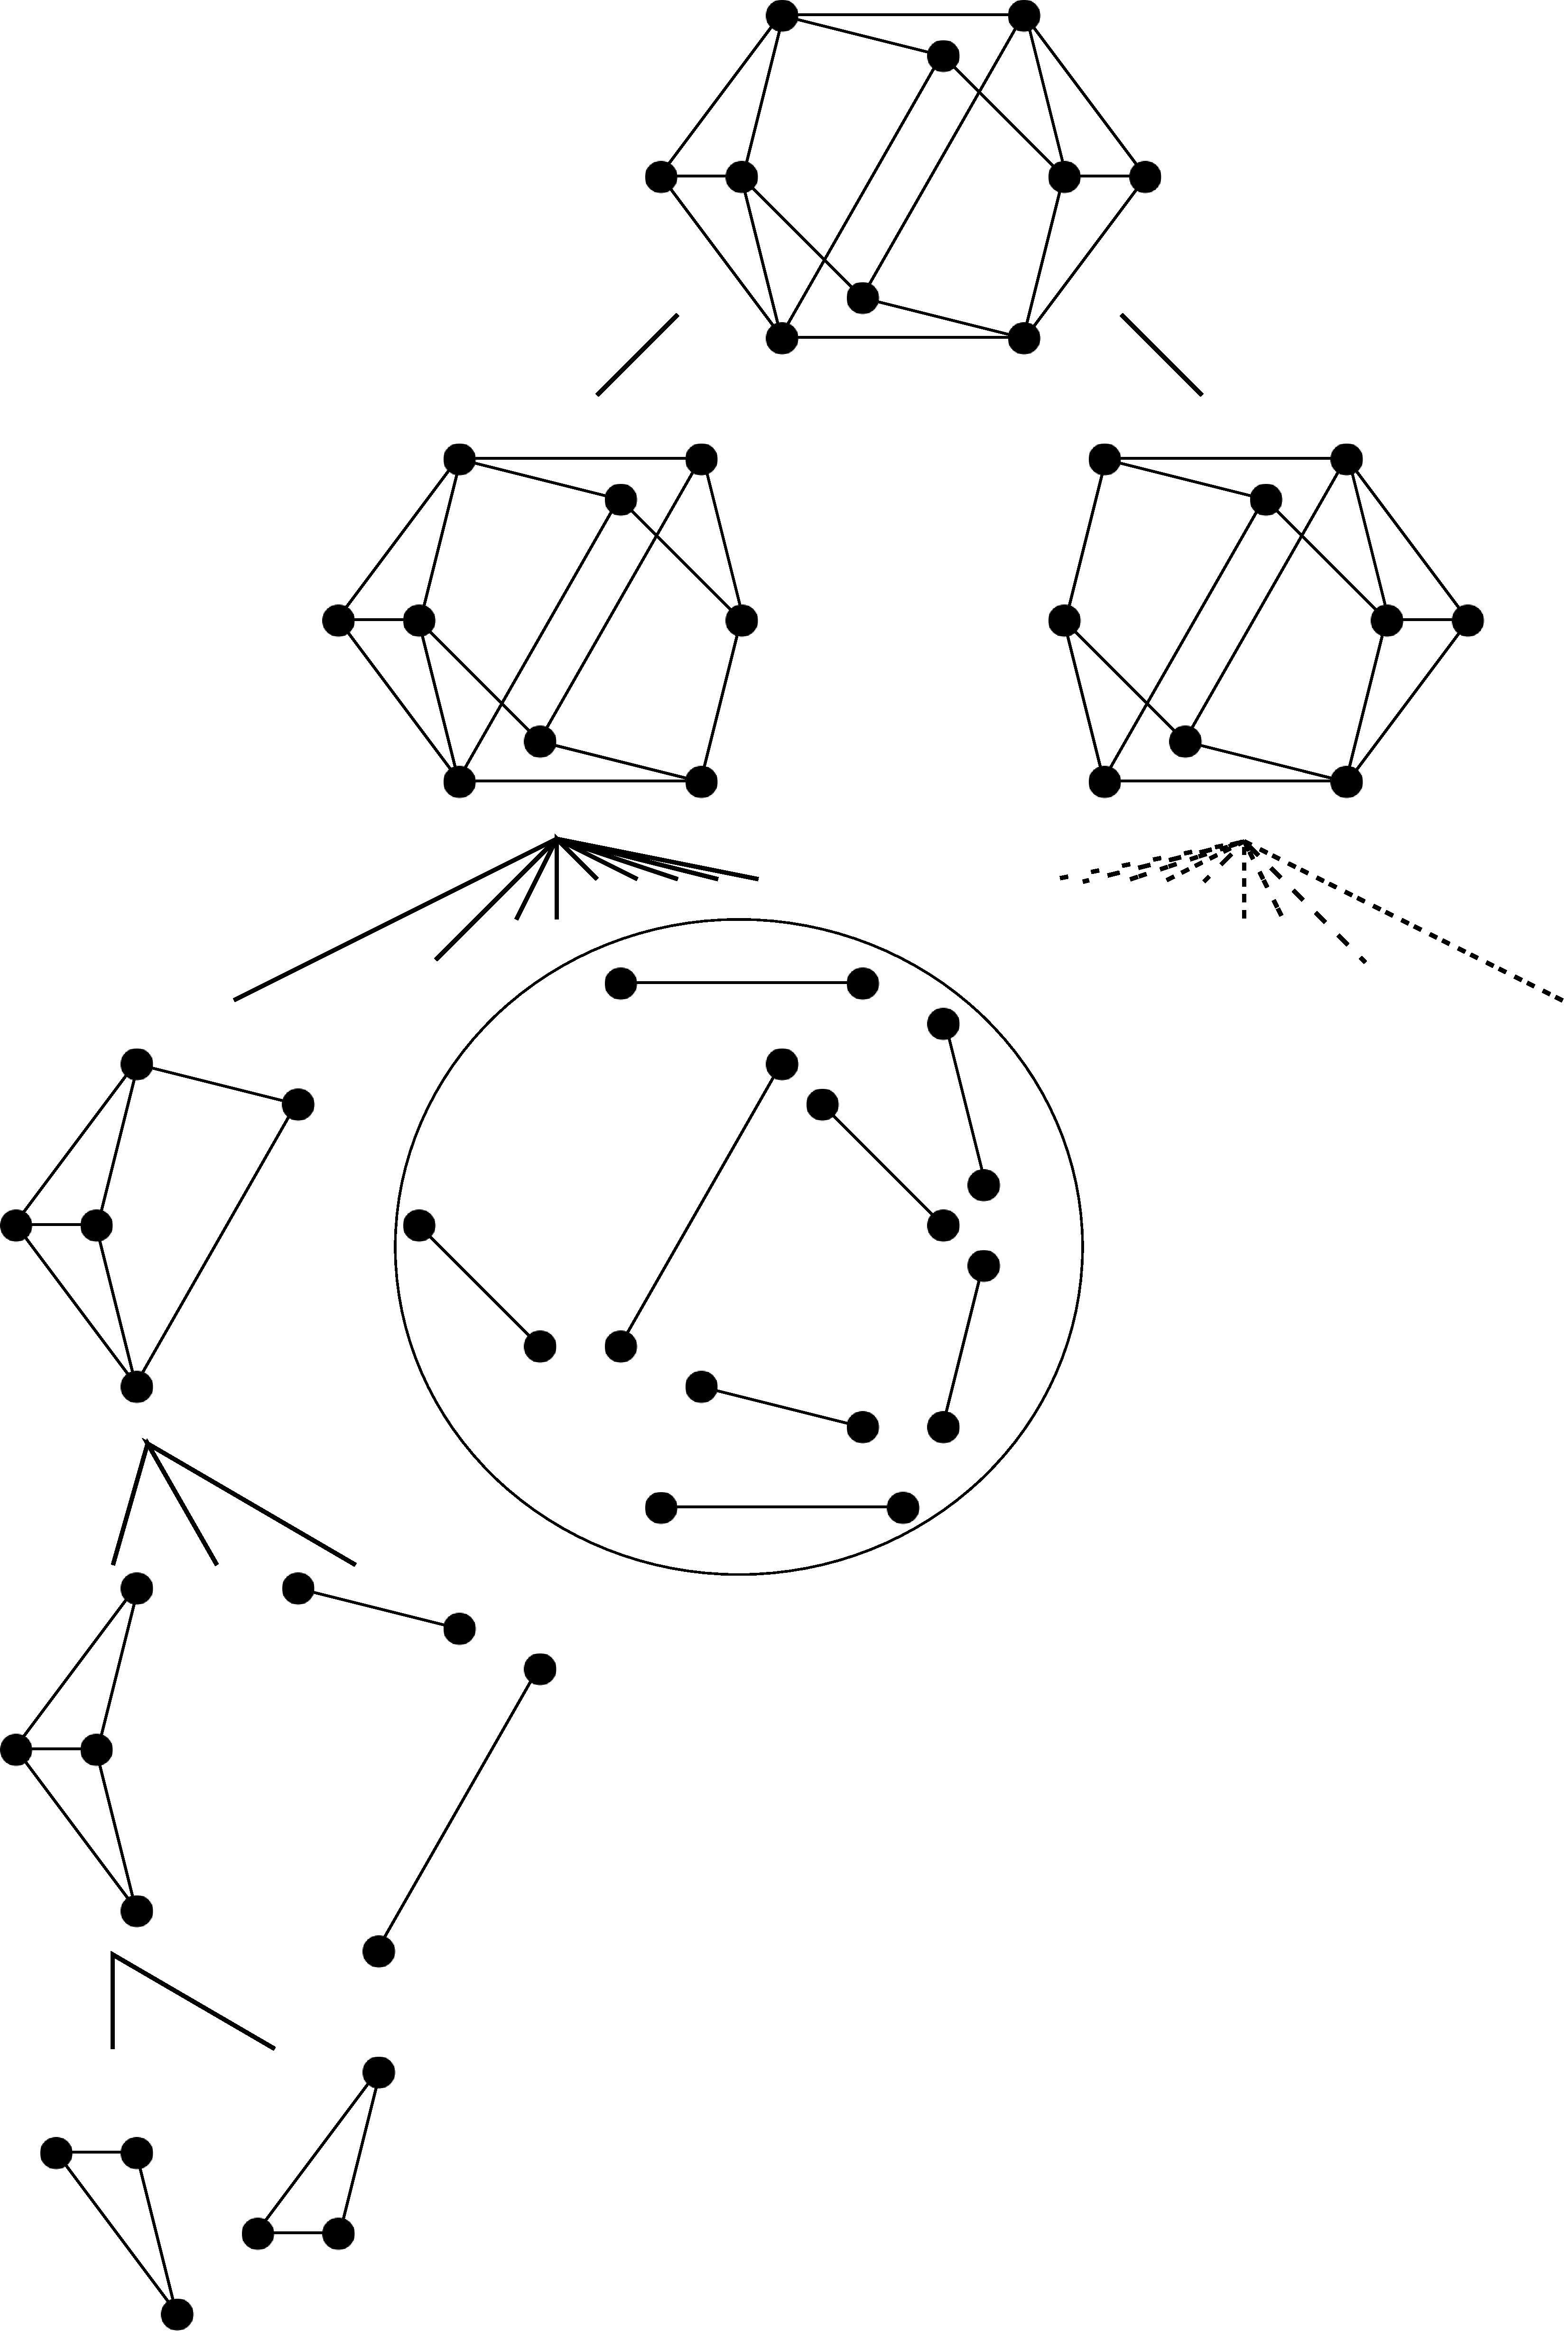
\includegraphics[width=\linewidth]{../../img/svg/new_overconstrained_not_optimal}
        \end{subfigure}
    \end{figure}

\end{frame}

\begin{frame}{Canonical DR-Plan}
    We show that one can avoid the NP-hardness of planning if the input linkage is independent (i.e.\ not overconstrained.)
\n
    We introduce a canonical DR-plan, which is guaranteed to exist and to be optimal for independent graphs.
\n

    % \begin{definition}
    %     The \dfn{canonical DR-plan} of an abstract rigidity matroid $\matroid=(K(V), \closure{\cdot})$ in $\RR^d$ satisfies the following three properties:
    %     \begin{enumerate}
    %         \item It is a DR-plan of $\matroid$;
    %         \item Children are closed proper subsets of the parent
    %         ($E_i=\left<E_i\right>$ and $E_i\subsetneq E$); and
    %         \item If all pairs of closed proper subsets intersect trivially (cardinality is $\leq d$, $|V(E_i) \cap V(E_j)| \leq d$) then all of them are children, otherwise exactly two that intersect non-trivially are children.
    %     \end{enumerate}
    % \end{definition}

    % \begin{definition}
    %     The \dfn{canonical DR-plan} satisfies the following three properties:
    %     \begin{enumerate}
    %         \item It is a DR-plan.
    %         \item Children induce maximal proper subsets of their parent's vertex set (i.e.\ they induce rigid vertex-maximal proper subgraphs of the parent.)
    %         \item If all pairs of viable children sets intersect trivially on their induced vertex set ($|V(F_i) \cap V(F_j)| < d$) then all of them are children, otherwise exactly two that intersect non-trivially are children.
    %     \end{enumerate}
    % \end{definition}

    \begin{definition}
        A \dfn{canonical DR-plan} is a DR-plan that satisfies the additional two properties:
        \begin{enumerate}
            \item Children are rigid vertex-maximal proper subgraphs of the parent.
            \item If all pairs of rigid vertex-maximal proper subgraphs intersect trivially then all of them are children, otherwise exactly two that intersect non-trivially are children.
        \end{enumerate}
    \end{definition}

    % \begin{definition}
    %     Let $C$ be the children of a node, and $P$ be the set of rigid vertex-maximal proper subgraphs of the same node. Then, a \dfn{canonical DR-plan} is a DR-plan that satisfies the additional property at every internal node: If $a,b\in P$ intersect trivially, then $P=C$; else, some two subgraphs $a, b\in P$ must satisfy $\set{a,b}=C$.
    % \end{definition}

    % While not unique, we show that any non-uniqueness doesn't effect optimality.
\end{frame}

\begin{frame}{Algorithm}
    Furthermore, we provide an $O(n^3)$ algorithm to find the canonical DR-plan, if the rigidity-related matroid is additionally a sparsity matroid.
\n
    As a byproduct, this also finds the minimum and maximum (non-trivial) rigid subgraphs of the input, which is NP-hard in general.
\end{frame}




% \begin{frame}{Further Contributions}
%     \begin{itemize}[<+->]
%         \item New notion of a canonical DR-plan, applicable to independent graphs in abstract rigidity matroids.

%         \item An $O(n^3)$ algorithm to find the canonical DR-plan, if independence in the abstract rigidity matroid is captured by a sparsity condition.

%         \item A new technique to quickly realize (or solve) constraint systems with indecomposable graphs, using recent results on Cayley configuration spaces.

%         \item Applications to
%         \begin{itemize}
%             \item 2D bar-joint [...]
%             \item 2D body-hyperpin (0-, 1-, and 2-dof) [Silica bilayers]
%             \item 2D pinned line-incidence systems [Crosslinked microtubules]
%         \end{itemize}
%     \end{itemize}
% \end{frame}

\begin{frame}{Material Modeling}
    Applications to other abstract rigidity matroids where independence corresponds to sparsity
    % we can model materials....
    \begin{itemize}
        \item 2D bar-joint [Cross-sections of microtubule structures and organic tissue with hierarchical structure]
        \item 2D body-hyperpin (0-, 1-, and 2-dof) [Silica bilayers]
        \item 2D pinned line-incidence systems\footfullcite{sitharam2014dictlearning} [Crosslinked microtubules]
    \end{itemize}

    \begin{figure}\centering
        %
        \begin{subfigure}{.24\linewidth}\centering
            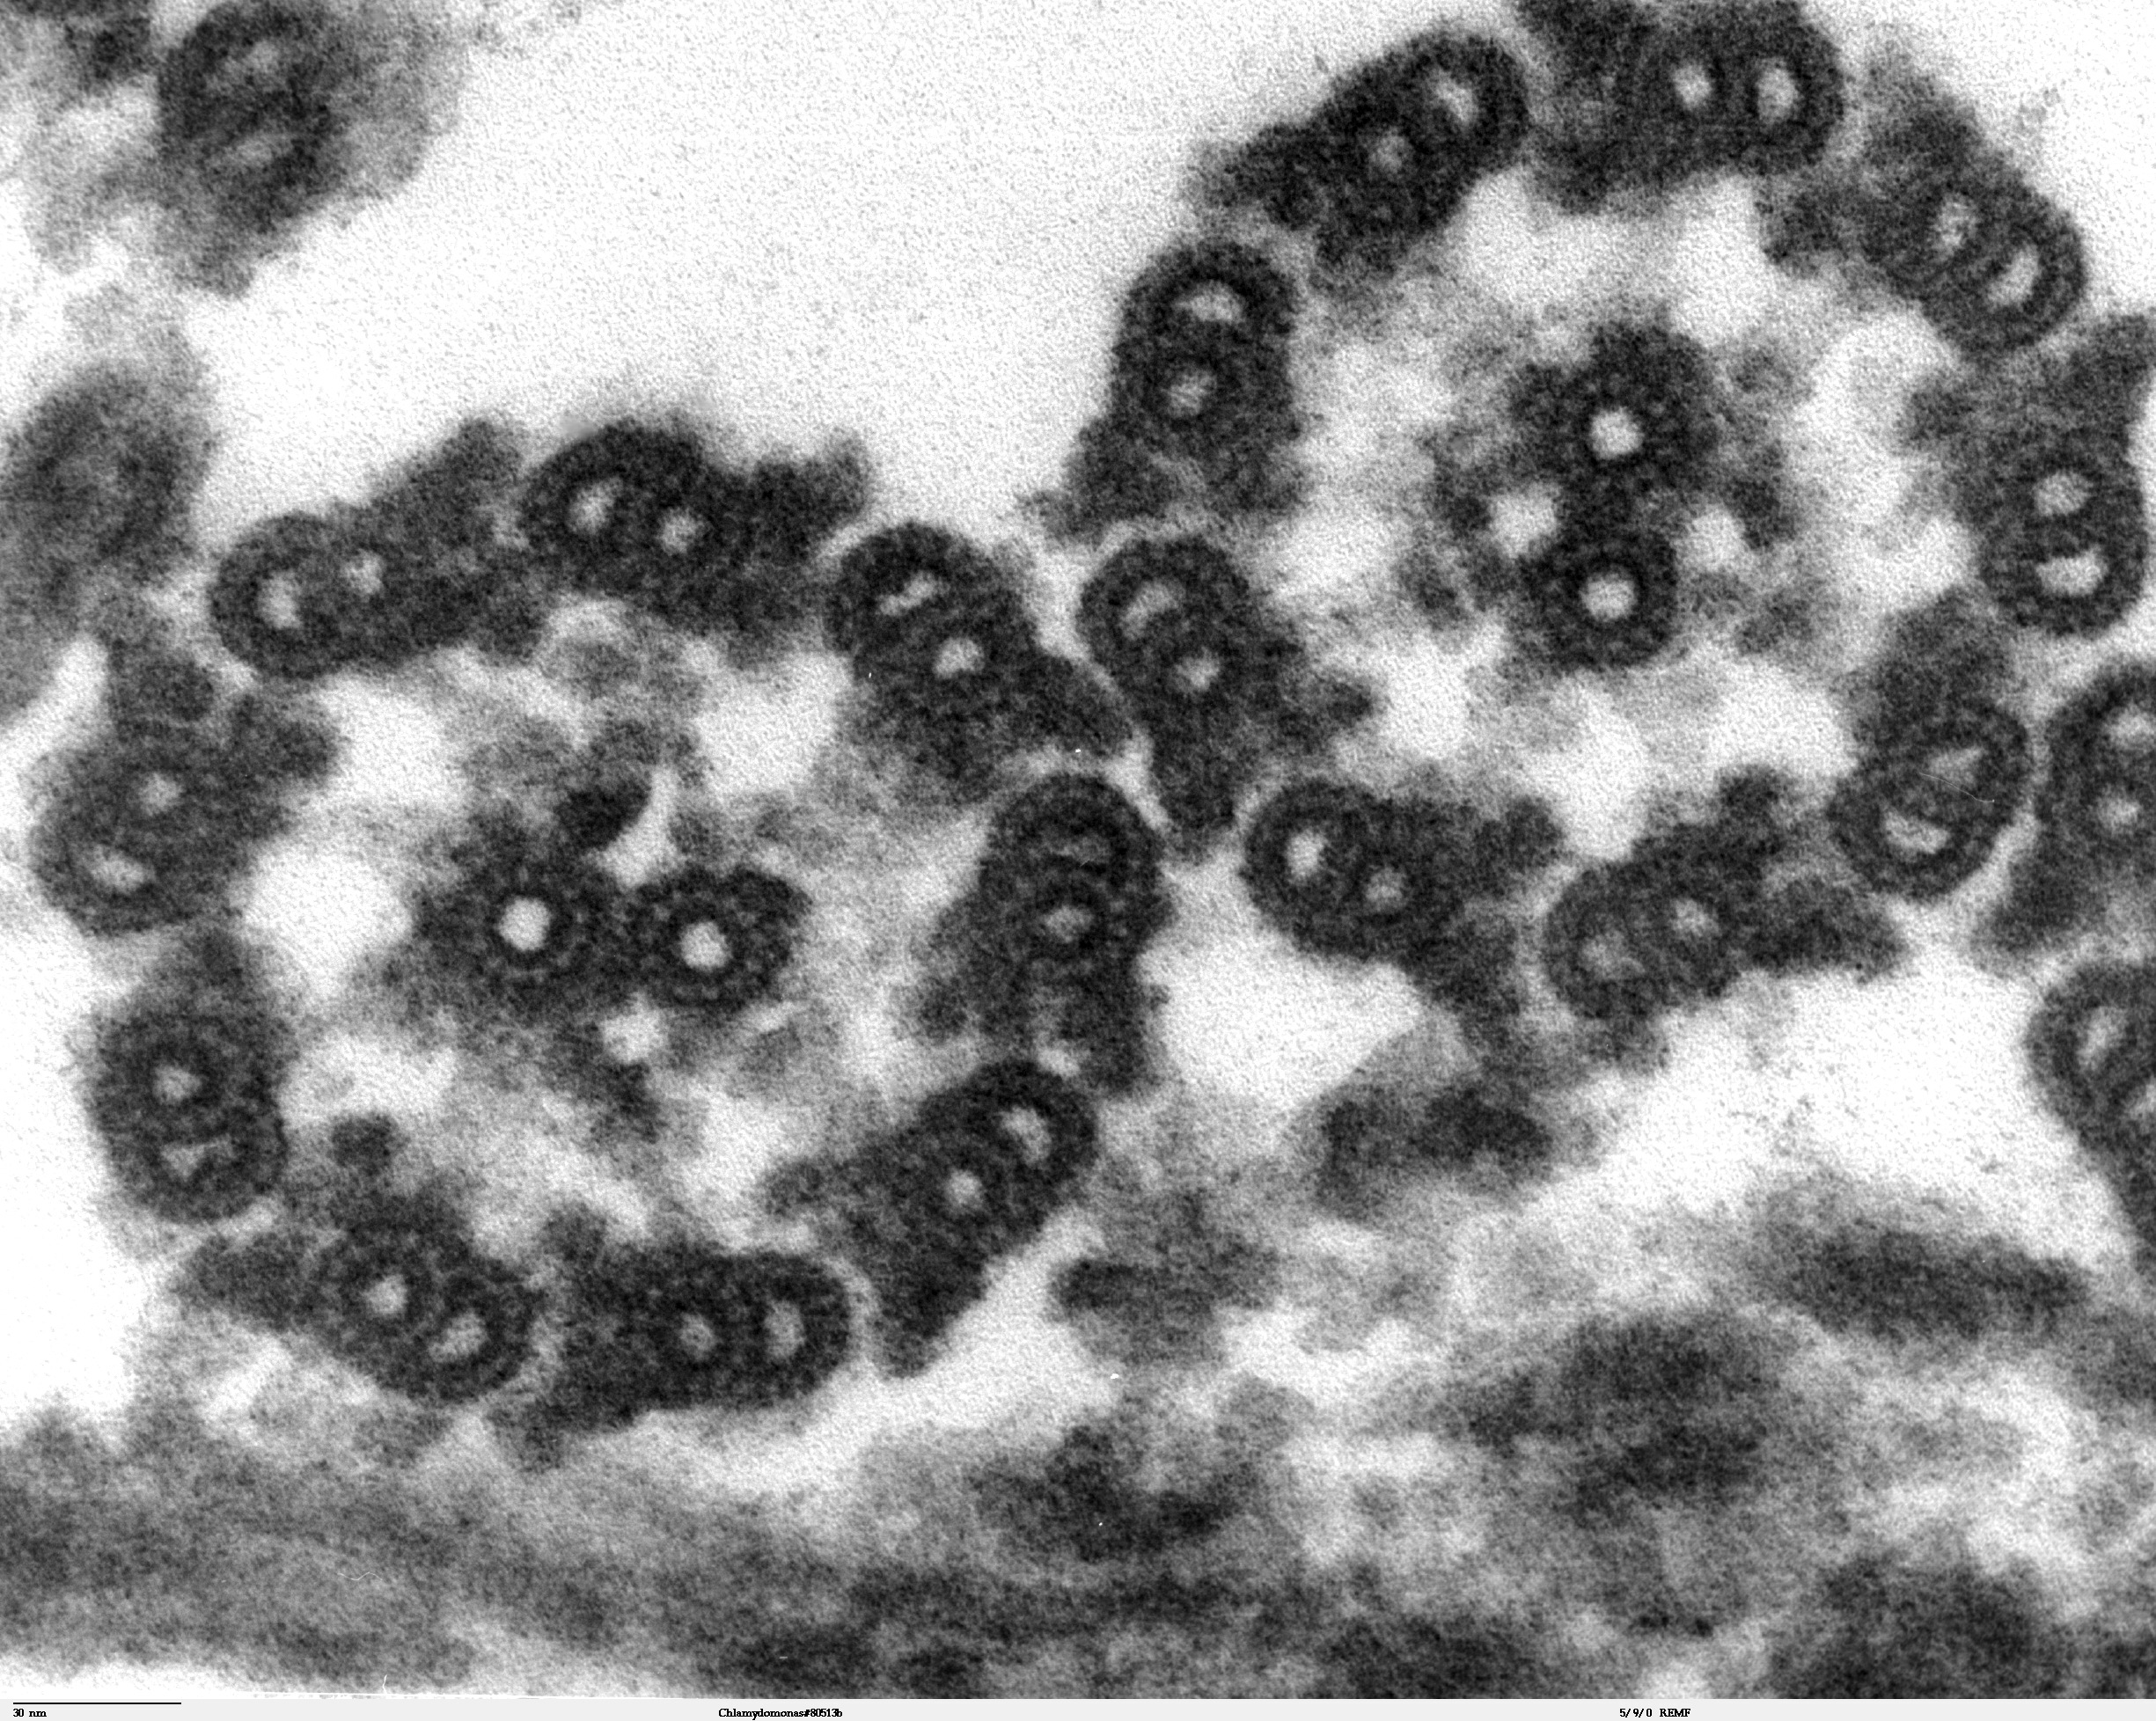
\includegraphics[width=\linewidth]{../../img/Chlamydomonas_TEM_17}
        \end{subfigure}
        %
        \hfill
        \begin{subfigure}{.24\linewidth}\centering
            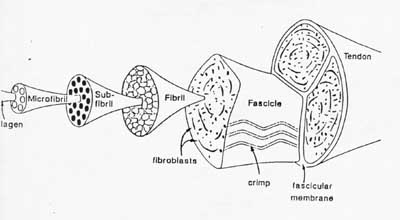
\includegraphics[width=\linewidth]{../../img/ligten2.jpg}
        \end{subfigure}
        %
        \hfill
        \begin{subfigure}{.24\linewidth}\centering
            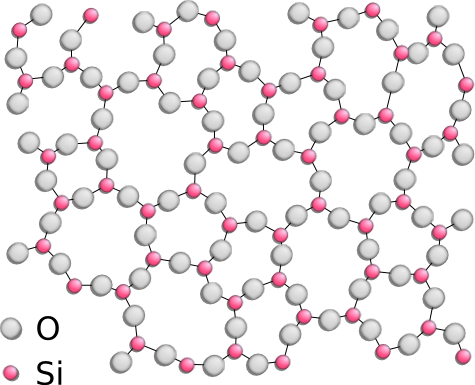
\includegraphics[width=\linewidth]{../../img/Silica}
        \end{subfigure}
        %
        \hfill
        \begin{subfigure}{.24\linewidth}\centering
            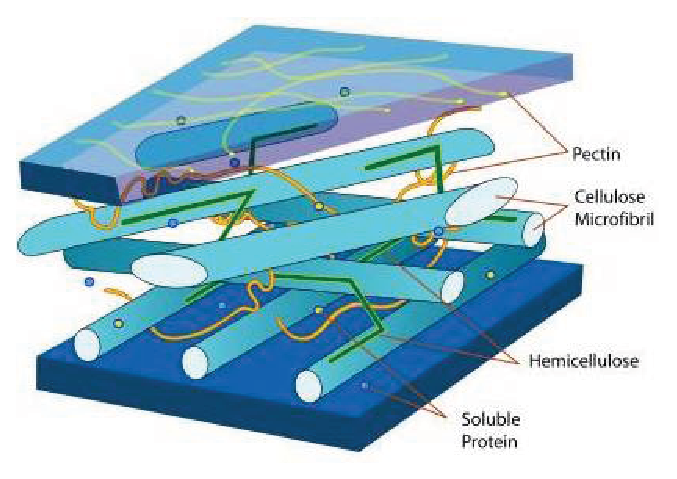
\includegraphics[width=\linewidth]{../../img/crosslink}
        \end{subfigure}
    \end{figure}
\end{frame}

\begin{frame}{Further Contributions}
    A new technique to efficiently realize indecomposable constraint systems (i.e.\ their optimal DR-plan has depth of 1), by optimal modification using recent results on Cayley configuration spaces.
\end{frame}

\begin{frame}{Open Source Software}
    Under development.\footfullcite{baker2015arxiv}

    Current version available at: \url{cise.ufl.edu/~tbaker/drp}
    \begin{figure}\centering
        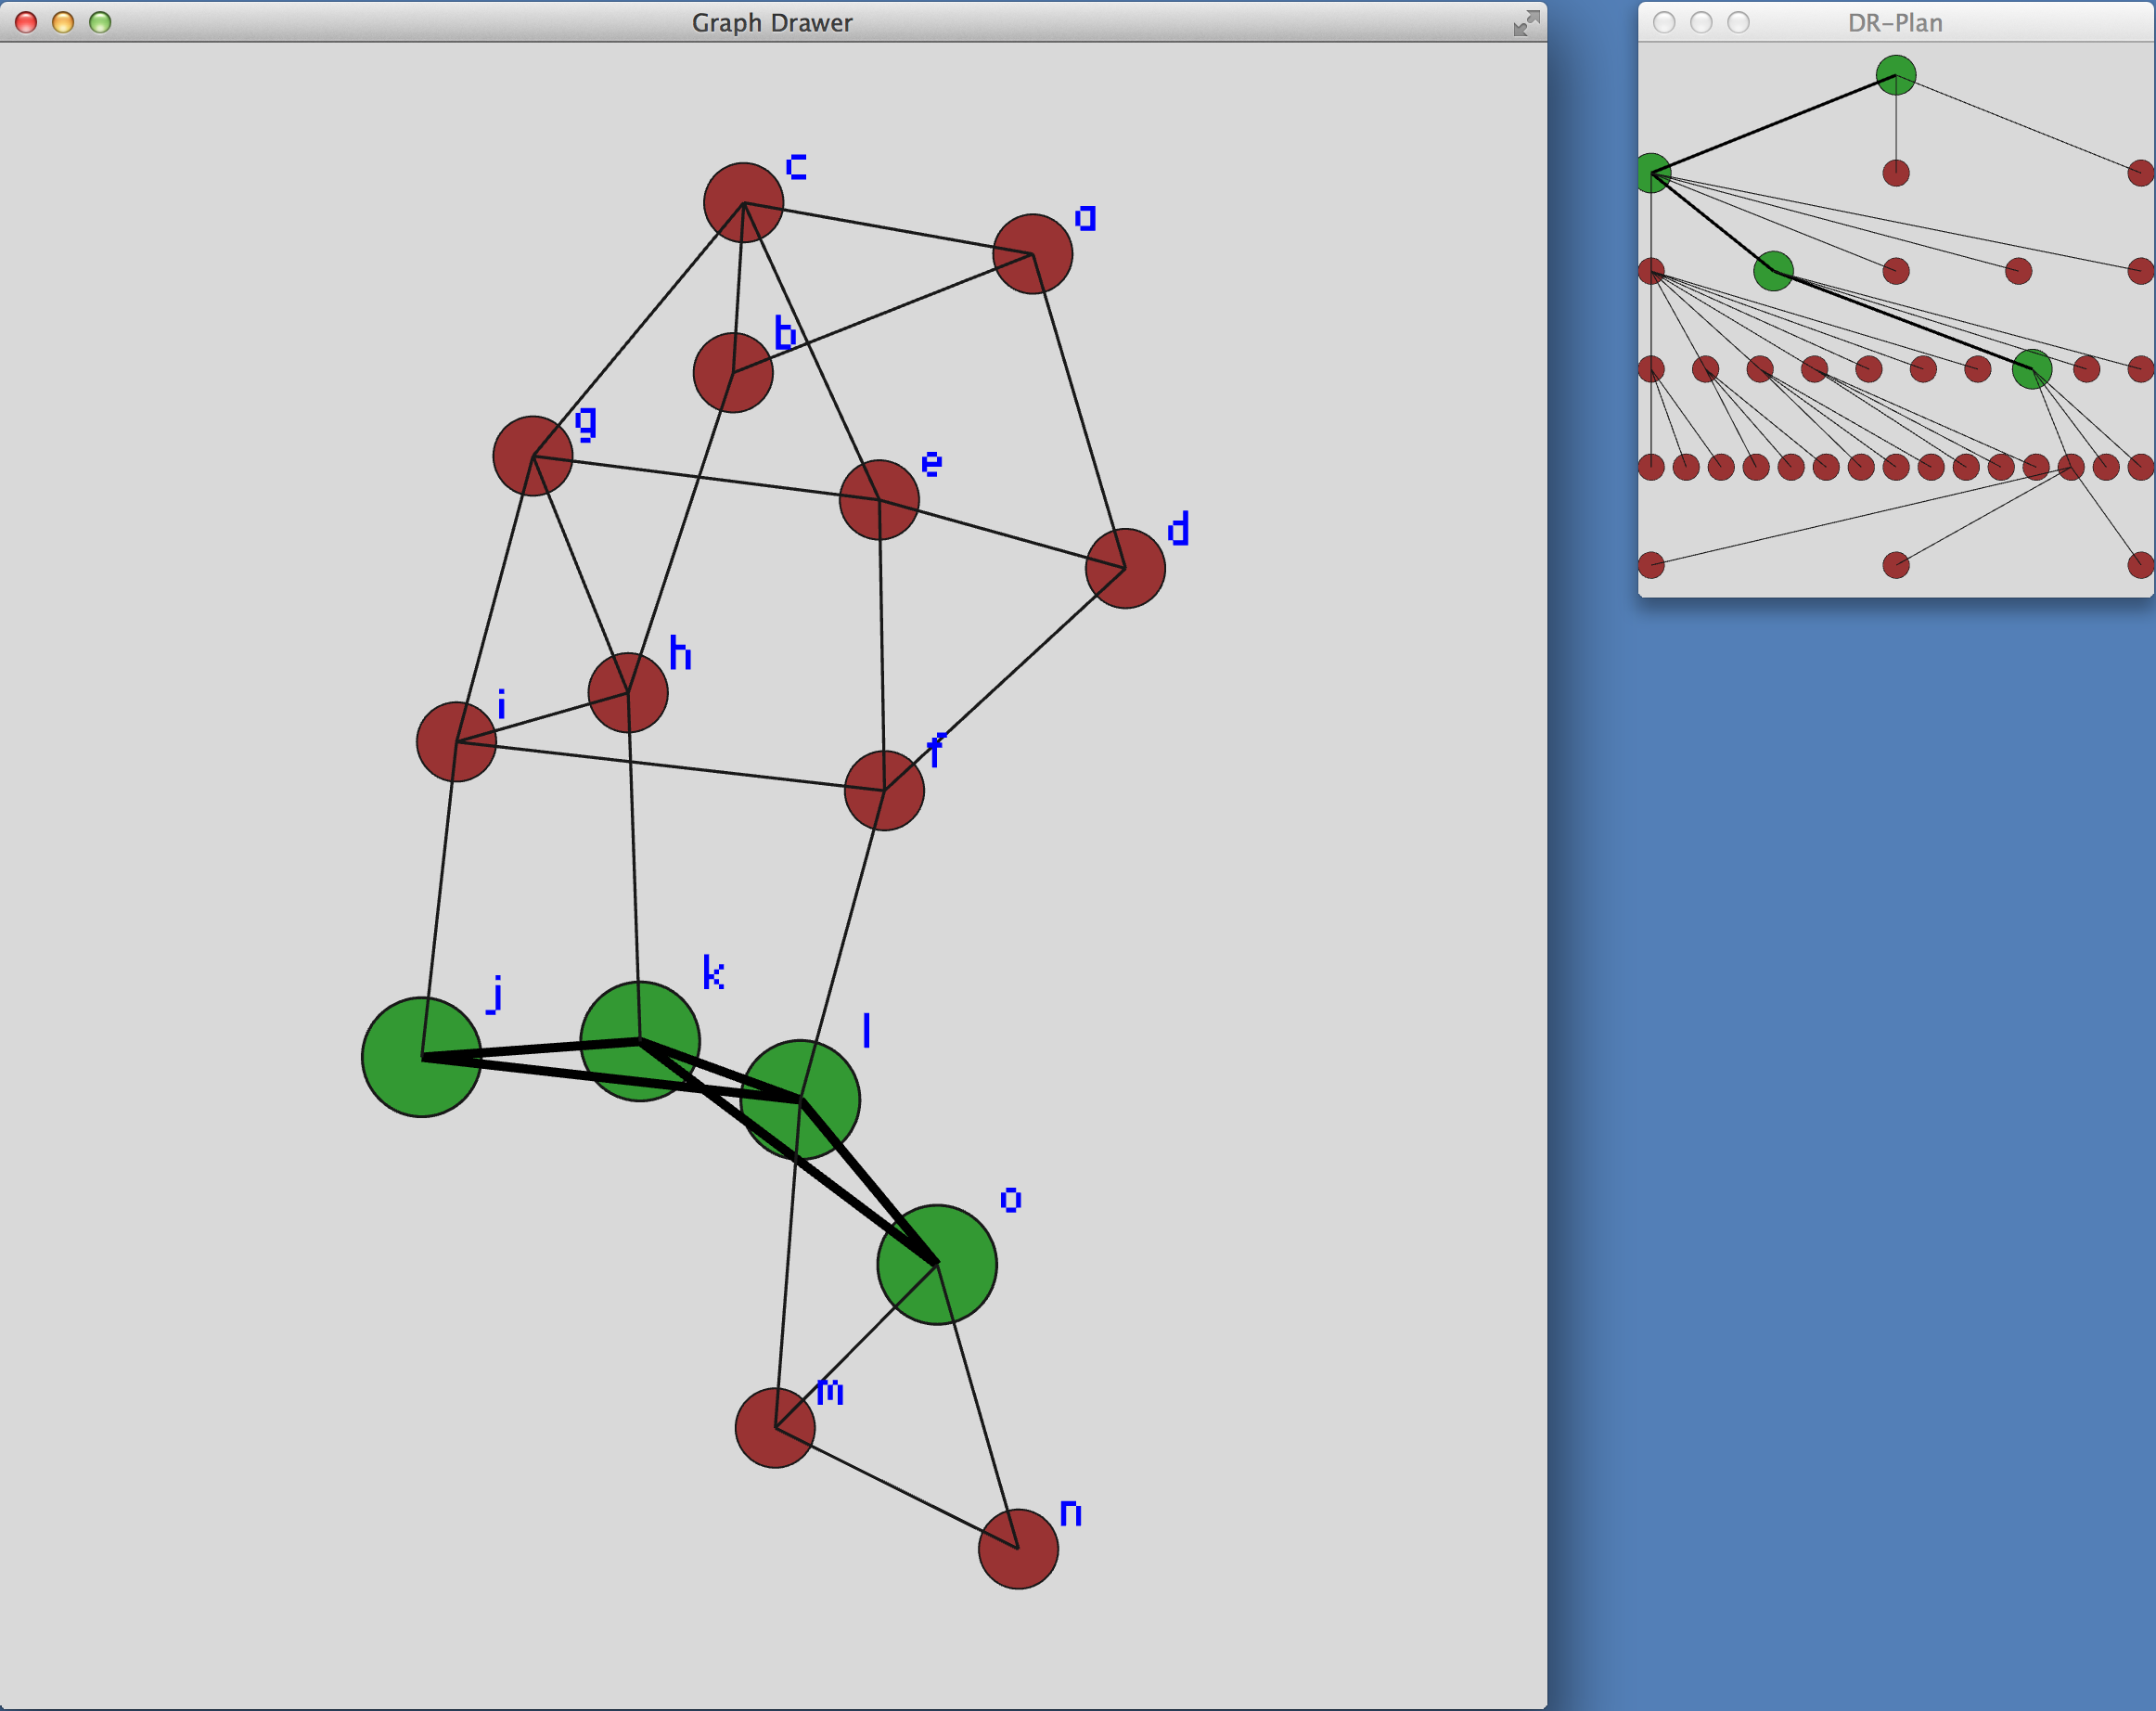
\includegraphics[width=0.65\linewidth]{../../img/screenshots/node_in_drp}
    \end{figure}
\end{frame}

\begin{frame}{Open Problems}
    \begin{openproblem}
        Is there a more efficient algorithm than $O(n^3)$ to find the canonical DR-plan of isostatic 2D bar-joint graphs?
    \end{openproblem}

    \begin{conjecture}
    \label{conj:mfaisoptimal:rephrase}
        For independent graphs, cluster-minimal DR-plans are optimal. In fact, for independent graphs, cluster-minimality and canonical are equivalent properties of a DR-plan.
    \end{conjecture}

    Additional problems can be found in the paper.
\end{frame}

% \begin{frame}{Open Problems, cont.}
%     % \footnotesize

%     \begin{openproblem}
%         For fixed $k$, we have polynomial time optimal DR-planning (Section~\ref{sec:DRP}), recombination (modification) in the presence of $k$ overconstraints, optimal modification for decomposition OMD$_k(G)$ when at most $k$ constraints are removed (Section~\ref{sec:recomb}), and also optimal completion using at most $k\le 2$ constraints in the body-pin and triangle-multipin cases for a somewhat different optimization of the DR-plan (Section~\ref{sec:table}). However, in the running time of all of these algorithms, $k$ appears in the exponent. Can $k$ be removed from the exponent?
%     \end{openproblem}

%     \begin{openproblem}
%         What is the complexity of the optimal completion problem when the given graph has more than 2-dofs? Our proof for the 1 and 2-dof cases relied heavily on the matroidal properties of their corresponding $(k,l)$-tightness. For higher number of dofs, the $(k,l)$ characterization is no longer matroidal \cite{Lee:2007:PGA}. As a result, the major obstacle is that there is no easy way of obtaining an optimal or canonical $k$-dof DR-plan in general. Even assuming such  a DR-plan is available, if higher dofs had the same characteristics, Observation \ref{obs:algebraic_completion} raises questions about the correct measure of DR-plan size that captures algebraic complexity for recombining graphs with many dofs (this is not an issue in the isostatic case). Unless some restrictions can be found and taken advantage of, the $k$-dof optimal completion problem would  have complexity exponential in $k$.
%     \end{openproblem}

%     \begin{openproblem}
%         What is the complexity of the restricted OMD (optimal modification for decomposition) problem? This has the potential to be difficult. For example, when the isostatic completion is required to be a 2-tree the restricted OMD problem is reducible to the maximum spanning series-parallel subgraph problem shown by \cite{cai1993spanning} to be NP-complete even if the input graph is planar of maximum degree at most 6. However, since the OMD problem has other input restrictions such as not having any proper isostatic subgraphs, it is not clear if the reverse reduction exists and hence it is unclear whether the OMD problem is NP-complete.

%         The same holds for the restricted OMD problem where the isostatic completion is required to be a tree-decomposable graph of low Cayley complexity (i.e.\ have special, small DR-plans). One potential obstacle to an indecomposable graph $G$'s membership in the restricted OMD$_k$ for small $k$ is if $G$ is tri-connected and has large girth. In fact, 6-connected (hence rigid) graphs with arbitrarily large girth have been constructed in \cite{servatius2000rigidity}.
%     \end{openproblem}

%     \begin{openproblem}
%         Is the OMD (optimal modification for decomposition) problem reducible to the OC (optimal completion) problem?
%     \end{openproblem}

% \end{frame}


% \begin{frame}\frametitle{End}
%     \tableofcontents
% \end{frame}







% \section{Old}

% \subsection{Definitions}
% \begin{frame}{Introduction}
%     This is a short introduction to Beamer class.
%     \pause
%     This is some more.
% \end{frame}


% \begin{frame}{Blocks}
%     \begin{block}{Block title}
%         This is a block in blue
%     \end{block}

%     \begin{definition}
%         Definition
%     \end{definition}

%     \begin{theorem}
%         Theorem
%     \end{theorem}

%     \begin{proof}
%         Proof
%     \end{proof}
% \end{frame}


% \begin{frame}{Test}
%     \begin{itemize}
%         \item<2-> appears from slide 2 on
%         \begin{itemize}
%             \item Sub list
%         \end{itemize}
%         \item<2-4> appears from slides 2-4
%         \item<4> appears on slide 4
%         \item<5-> appears from slide 5 on
%     \end{itemize}

%     \uncover<4-5>{
%         Appear from slides 4-5
%     }

%     \invisible<2>{HI!} \alt<2>{BYE!}{oops}
%     \alert<2>{Red words on slide 2.} \color<2>{green}{Green words on slide 2.} %remove #s to make always alert or green


%     \begin{itemize}
%         \item Language used by Beamer: L\uncover<2->{A}TEX
%         \item Language used by Beamer: L\only<2->{A}TEX
%     \end{itemize}

%     \begin{enumerate}[<+-| alert@+>]
%         \item L
%         \item A
%         \item T
%         \item E
%         \item X
%         \item !
%         \begin{enumerate}
%             \item Sub items
%         \end{enumerate}
%     \end{enumerate}
% \end{frame}

% \subsection{Sub nothing}
% \begin{frame}{What?}
% \end{frame}

% \section{Nothing}
% \begin{frame}{do?}
% \end{frame}

% \subsection{Sub nothing2}
% \begin{frame}{you want?}
% \end{frame}

% --------------------------------------------------------------
%                        End of Body
% --------------------------------------------------------------

\end{document}

% --------------------------------------------------------------
%                       End of Document
% --------------------------------------------------------------
